
\documentclass[10pt]{article}
\usepackage[utf8]{inputenc}
\usepackage{graphicx}
\usepackage{amsmath, amssymb}
\usepackage{geometry}
\usepackage{caption} 
\geometry{a4paper, margin=0.5in, landscape} 

\begin{document}

\section*{Comparative EIS Kinetics Report}
\textbf{Model Structure:} \texttt{R0-p(R1-p(R2,CPE2),CPE1)} \\
\textbf{Used data:} altered data, first 6 points removed and points with $freq > 2e+04$ removed

\begin{center}
    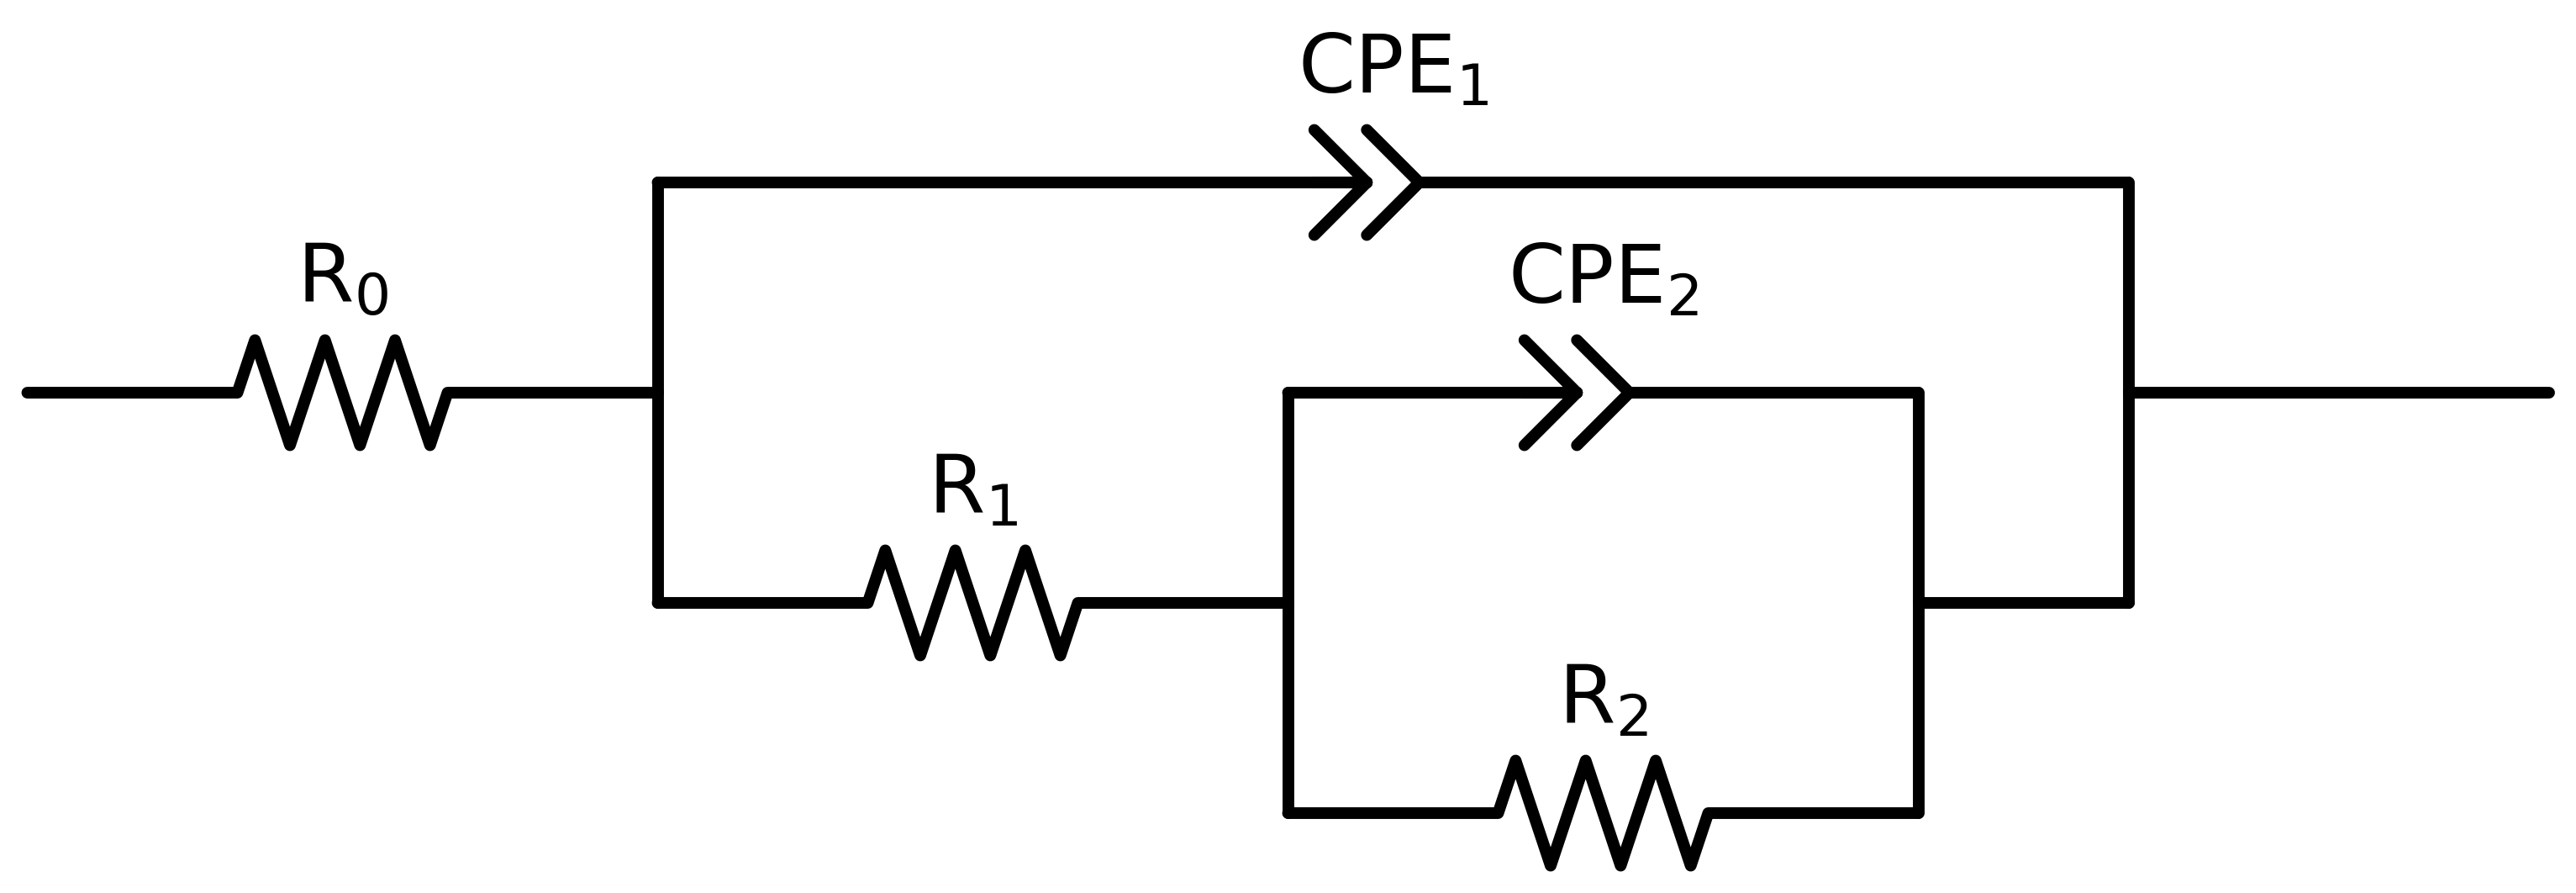
\includegraphics[width=0.45\textwidth]{../../2RC.png}
\end{center}

\renewcommand{\arraystretch}{1.6} 
\begin{table}[h!]
    \centering
    \footnotesize
    \begin{tabular}{|l|c|c|c|c|c|}
        \hline
        \textbf{Element} & \textbf{Unit} & \textbf{Bounds} & \textbf{Cauvel\_1\_MBT\_1H} & \textbf{Cauvel\_1\_MBT\_4H} & \textbf{Cauvel\_1\_MBT\_8H} \\ \hline
        $R_{0}$ & $\Omega$ & $[1.0e-03, 1.0e+03]$ & $8.12e+01 \pm 5.9e-01$ & $7.70e+01 \pm 4.4e-01$ & $7.58e+01 \pm 4.1e-01$ \\ \hline
        $R_{1}$ & $\Omega$ & $[1.0e+00, 1.0e+08]$ & $3.55e+05 \pm 7.6e+03$ & $5.25e+05 \pm 2.4e+04$ & $1.07e+03 \pm 4.1e+04$ \\ \hline
        $R_{2}$ & $\Omega$ & $[1.0e+00, 1.0e+08]$ & $2.92e+01 \pm 7.6e+03$ & $1.00e+08 \pm 4.3e-03$ & $7.68e+05 \pm 4.1e+04$ \\ \hline
        $Q_{2}$ & $\Omega$$^{-1}$ sec$^{a}$ & $[1.0e-11, 1.0e-03]$ & $4.40e-10 \pm 4.7e+01$ & $4.77e-05 \pm 1.7e-05$ & $5.60e-07 \pm 1.8e-07$ \\ \hline
        $n_{2}$ & - & $[5.0e-01, 1.0e+00]$ & $6.66e-01 \pm 1.2e-12$ & $1.00e+00 \pm 2.4e-01$ & $5.00e-01 \pm 2.7e-01$ \\ \hline
        $Q_{1}$ & $\Omega$$^{-1}$ sec$^{a}$ & $[1.0e-11, 1.0e-03]$ & $6.07e-06 \pm 2.4e-07$ & $6.67e-06 \pm 4.7e-08$ & $6.64e-06 \pm 3.0e-07$ \\ \hline
        $n_{1}$ & - & $[5.0e-01, 1.0e+00]$ & $9.28e-01 \pm 5.0e-03$ & $9.15e-01 \pm 1.4e-03$ & $9.15e-01 \pm 5.0e-03$ \\ \hline
        \textbf{$\chi^2$} & - & -  & $6.871e-04$ & $4.624e-04$ & $3.330e-04$ \\ \hline

    \end{tabular}
\end{table}


\newpage
\section*{Analysis Results: 1H}
\begin{center}
    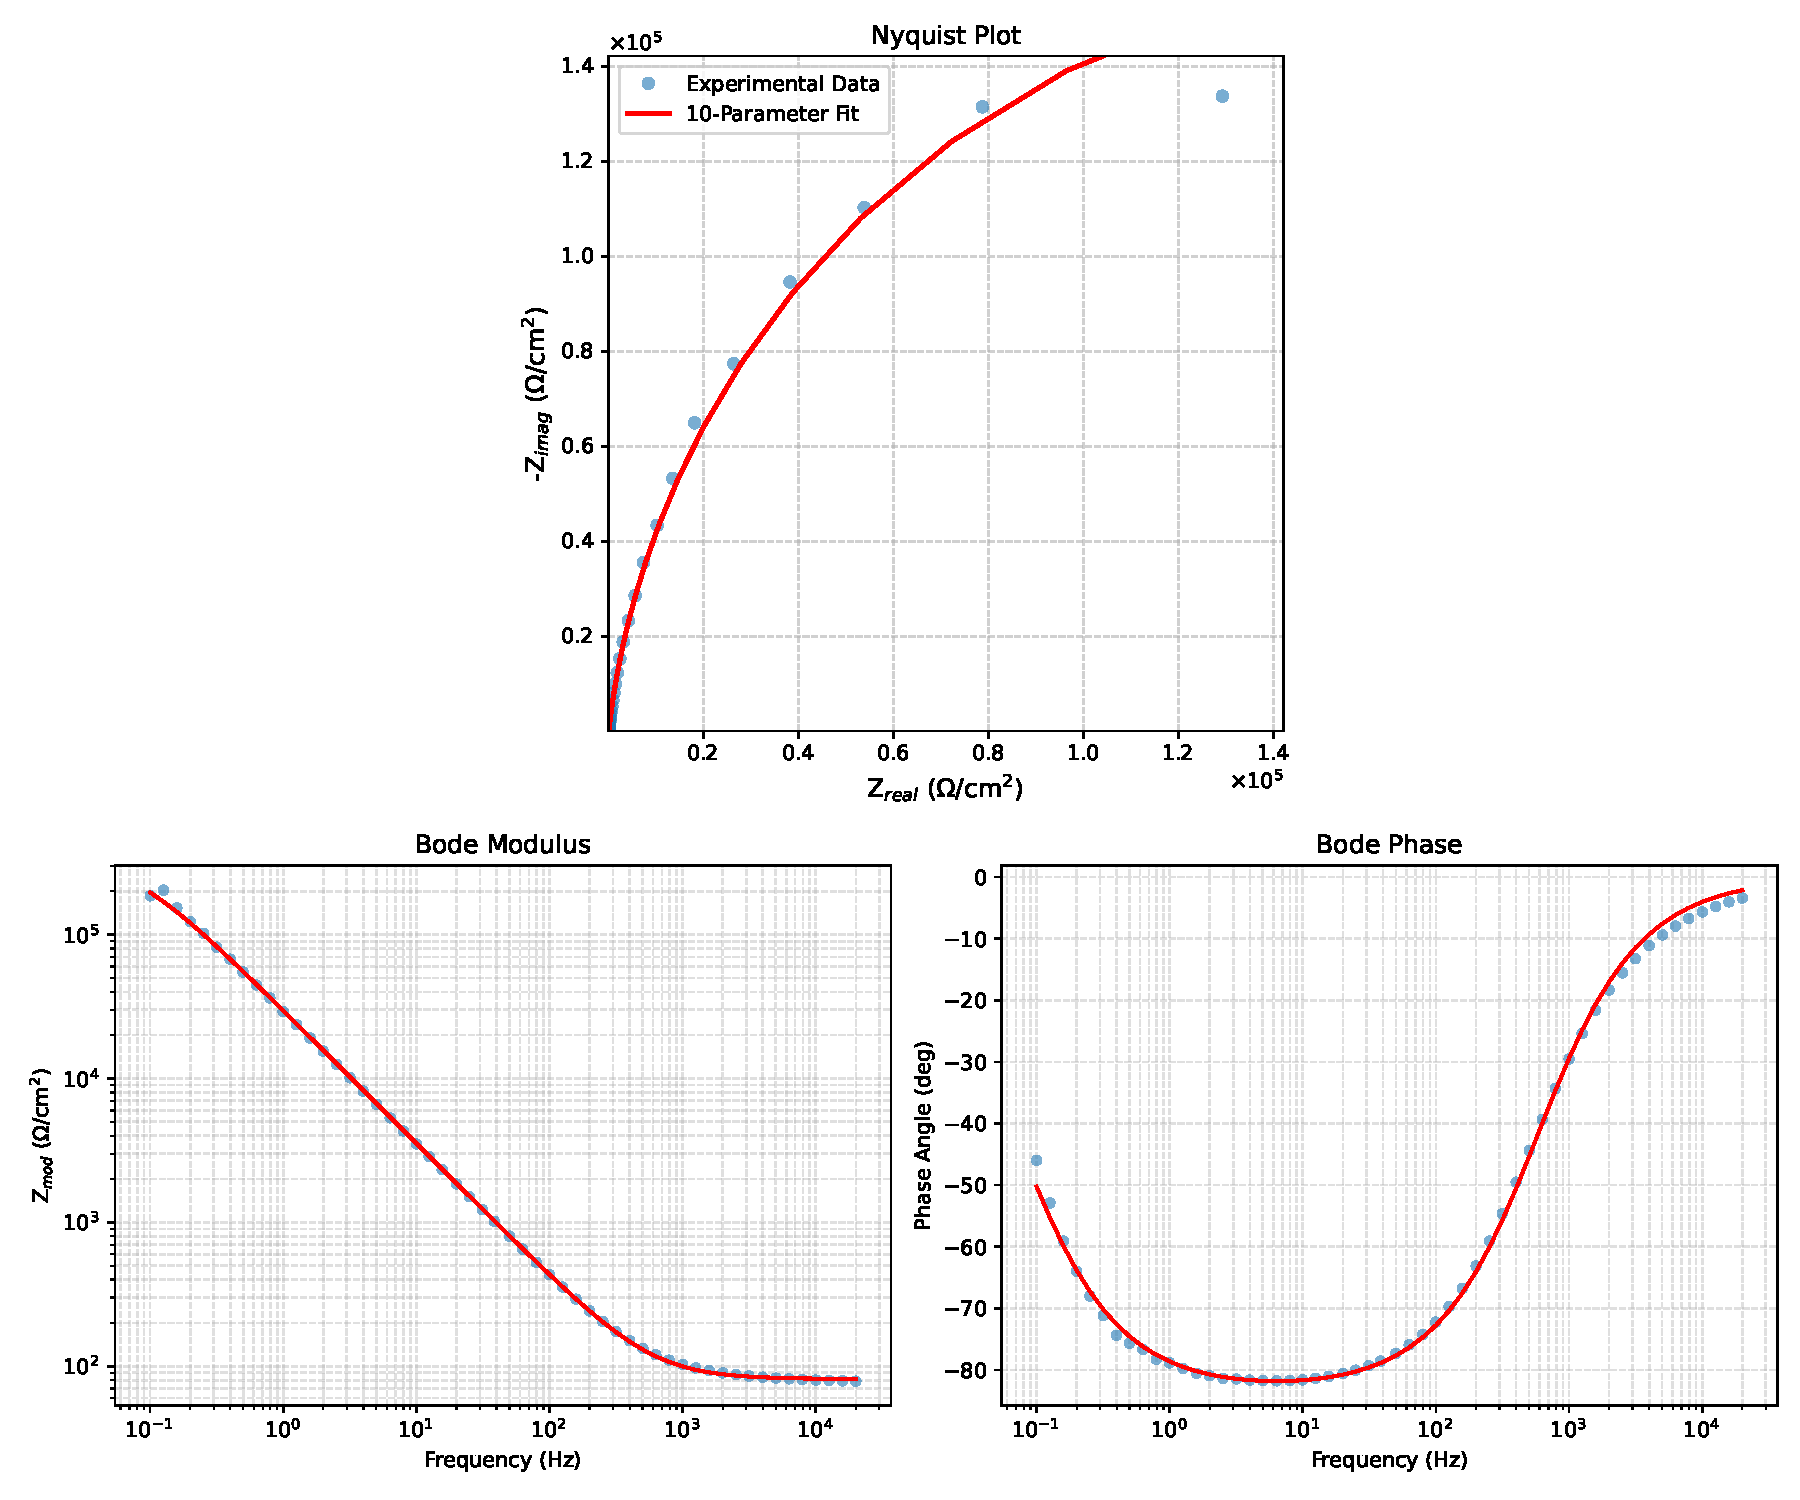
\includegraphics[width=0.7\textwidth]{plots_Cauvel_1_MBT_1H_2RC.pdf}
    \captionof{figure}{EIS Fit Results for Cauvel\_1\_MBT\_1H}
\end{center}

\newpage
\section*{Analysis Results: 4H}
\begin{center}
    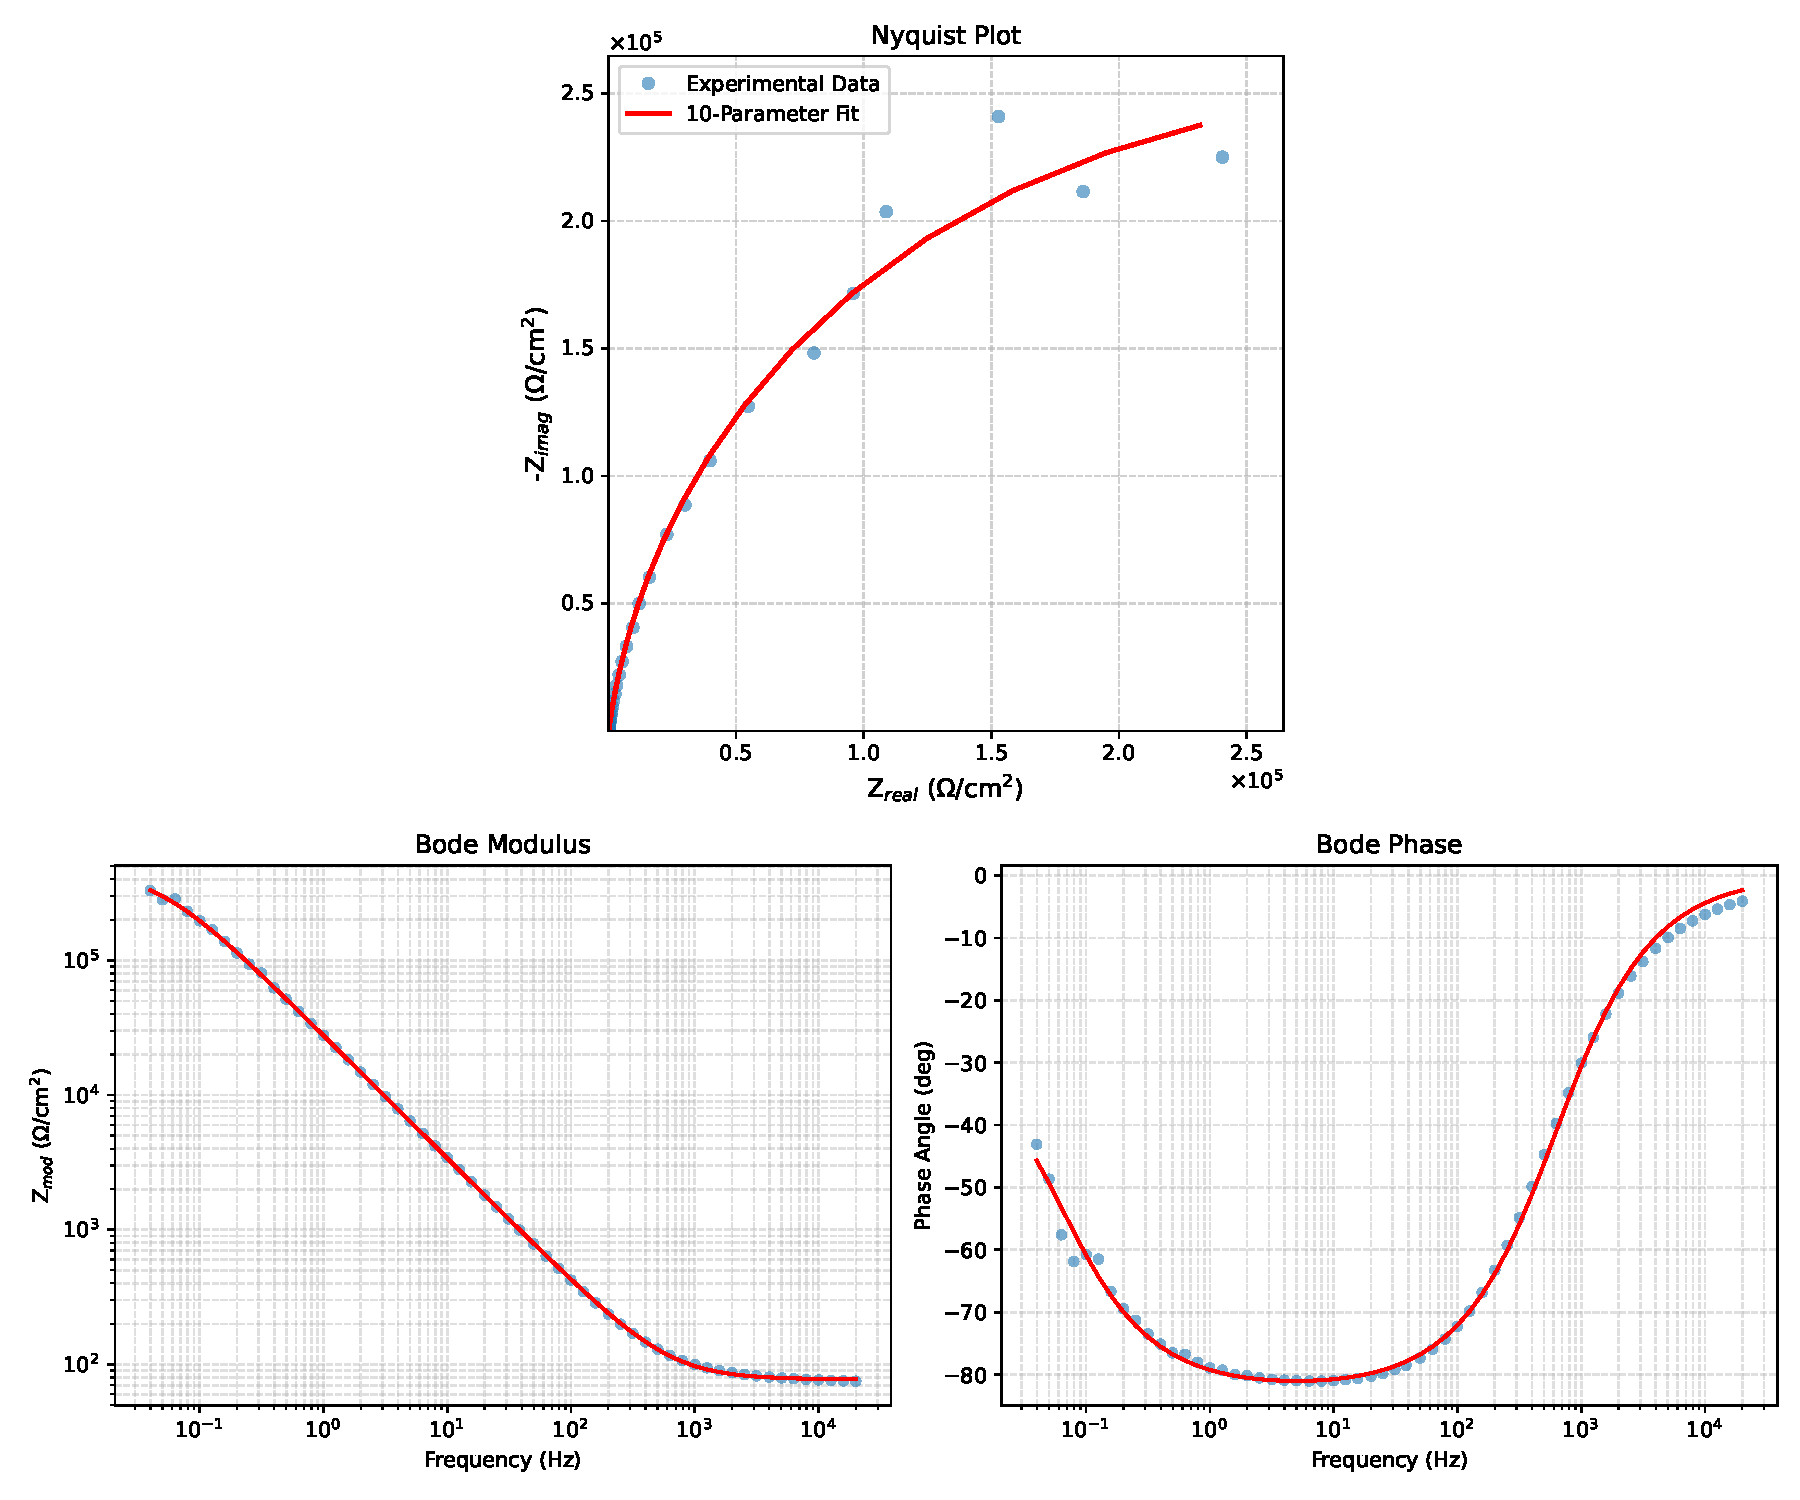
\includegraphics[width=0.7\textwidth]{plots_Cauvel_1_MBT_4H_2RC.pdf}
    \captionof{figure}{EIS Fit Results for Cauvel\_1\_MBT\_4H}
\end{center}

\newpage
\section*{Analysis Results: 8H}
\begin{center}
    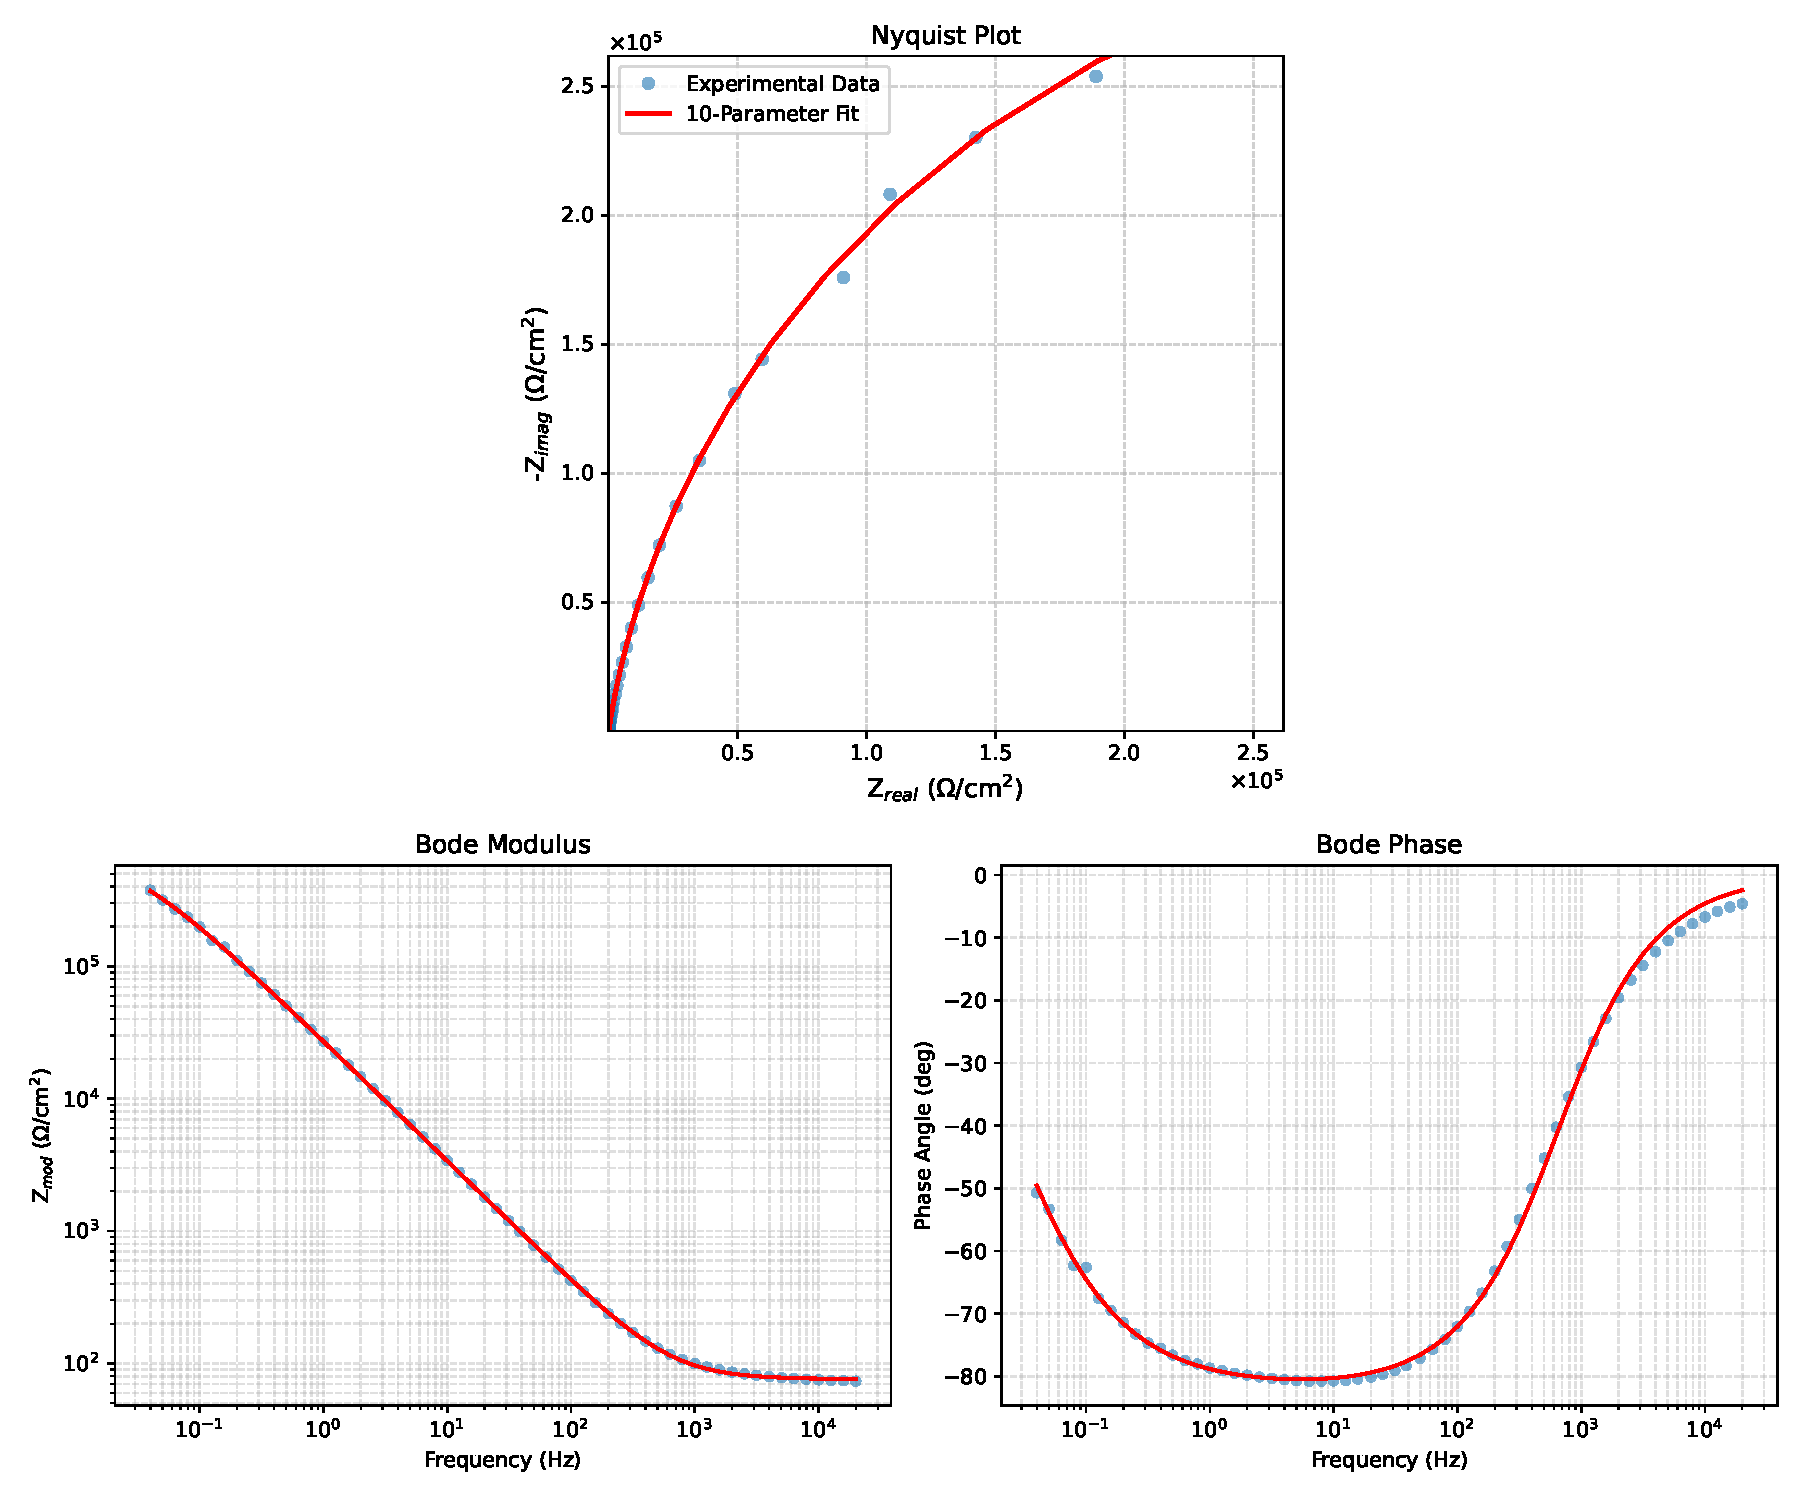
\includegraphics[width=0.7\textwidth]{plots_Cauvel_1_MBT_8H_2RC.pdf}
    \captionof{figure}{EIS Fit Results for Cauvel\_1\_MBT\_8H}
\end{center}


\end{document}
